\documentclass[pdftex,10pt,a4paper,oneside]{article}
%Can change the pt, papersize etc.
\usepackage{listings}
\usepackage{amsmath}
\usepackage{amssymb}
\usepackage{algorithm}
\usepackage{algorithmic} %Algorithm styles, need to be nested for the example shown
\usepackage{fancyhdr} %For our headers
\usepackage{graphicx} %Inserting images
\usepackage{lipsum}  %Blank text fill, delete me when finished
\usepackage{setspace} %Spacing on the front page for crest and titles
\usepackage[]{fncychap} % Styles can be Sonny, Lenny, Glenn, Conny, Rejne, Bjarne and Bjornstrup
\usepackage[hyphens]{url} %Deals with hyphens in urls to make them clickable
\usepackage{xcolor} %Great if you want coloured text
\usepackage{tabularx}
\usepackage{appendix} %Take a wild guess slick

%KEEP THIS ONE LAST it's quite buggy, it allows you to click on links within the pdf and web links without changing the colour. The mouse cursor simply changes its icon to indicate to the user. Great tool - still awkward
\usepackage[hidelinks]{hyperref}


%This will tell the compiler to do the header style, page and spacing between the header and text
\fancyhf{}
\renewcommand{\headrulewidth}{0.2pt}




% Load the package
\usepackage[toc]{glossaries}

% Generate the glossary
\makeglossaries
%\includeonly{%chapters/ch1.tex,
%	chapters/ch3.tex,
%	chapters/ch4.tex,
%	chapters/ch5.tex,
%	chapters/ch6.tex,
	%chapters/ch7.tex,
	%chapters/ch8.tex,
	%chapters/ch9.tex,
	%chapters/ch10.tex,
%	chapters/ch11.tex,
%	chapters/ch12.tex,
	%chapters/ch13.tex,	}
\begin{document}
	
	\pagenumbering{arabic}
	
	\begin{spacing}{2}
		\begin{center}
			
\includegraphics[scale = 0.20]{ASU.png}
		\end{center}
		\vspace{5mm}
		\begin{center}
			\textbf{\begin{LARGE}
					Conan:Finding missing people
			\end{LARGE}}
			\vspace{2mm}
		\end{center}
		\begin{center}
			\textbf{\large Mohamed Atta Ibrahim \\Mohamed Yasser Ahmed 
				\\Mahmoud Mohamed Benyamin \\ Hady Ashraf Ragab\\Yousef Abdelbadea Ali}
			\vspace{2mm}
		\end{center}
		\begin{center}
			\textbf{\large Supervisor:Dr. Mahmoud Khalil
			 }\\
			\textbf{\large Department of Computer and Systems Engineering}\\
			\textbf{\large Faculty of Engineering at Ain Shams University}\\
			
			{\large \today\\}
		\end{center}
	\end{spacing}
	
	\pagebreak
	
	\tableofcontents
	\pagebreak
	\listoffigures
	\pagebreak
	\listoftables
	\pagebreak
	\begin{abstract}{
			This paper presents imp DIP project
	}	\end{abstract}
	\pagebreak
	\section*{Introduction}
In this project the user can find missing people by search with the old pictures or young pictures of missing people. The project uses techniques that extract features from the pictures and check similarity between the query picture and the pictures in the dataset to retrieve the similar picture to the query picture.
	 
	\addcontentsline{toc}{section}{Introduction}
	
	
	\pagebreak
	
	\section{project description}
	This is a python desktop application, it applies the Pattern Recognition and	Digital Image Processing
	 techniques to analyze, design, and implement multimedia retrieval system, where the media that we are going to use are the images .we have implemented many techniques belong  Pattern Recognition and Digital Image Processing and AI techniques in retrieval and face Recognition.
	 .
	\begin{figure}[H]
		\centering
		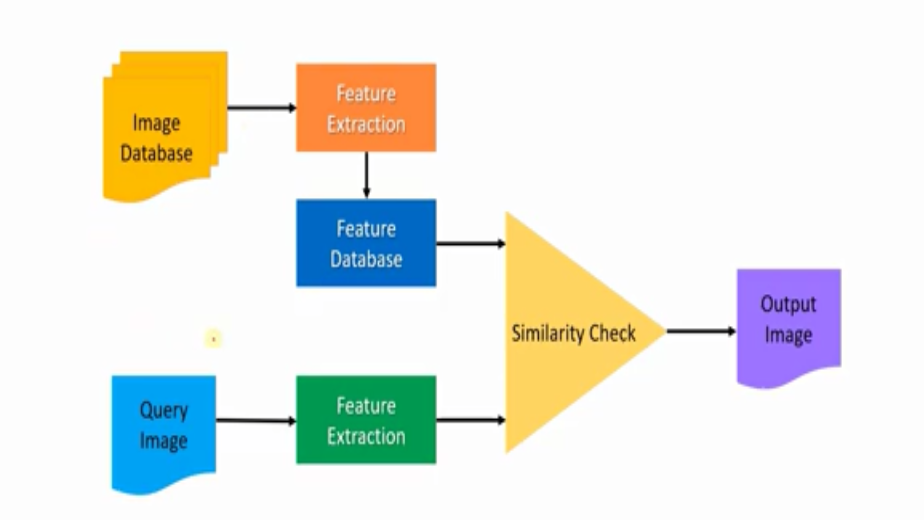
\includegraphics[width=120mm,height=60mm]{fig/19.png}
		\caption{image system block diagram }
		\label{image system block diagram}
	\end{figure}

	\pagebreak
	\section{Beneficiaries of the project}
	The family who want to find any one of their members because of missing of him.
	Any one who the government wants to find from his traffic camera's pictures to detect his data and find him.

	
	\pagebreak
	\section{Detailed analysis}
	This project deals with Content Based video Retrieval (CBVR)and Content Based Image Retrieval(CBIR). 
	For the CBIR, the adopted methods are color-based technique, texture-based technique, and shape-based technique. and then after the user select a technique and provide the image that he/she want to search for. The program extract features of the images dataset and save it then extract the features of the input image and compare the image with etracted feature database using the selected technique and by chi-squared distance. The chi-squared distance is distance measures that used to measures dissimilarity between two histograms. the following is an analysis for adopted technique in CBIR.

some distance that we used to measure similarity 
\begin{itemize}
	\item Absolute Distance \\
	\begin{equation}
		D_{Absolute}(h,\bar{h})= \sum_{K-1}^{K} |h_{K}-\bar{h_{K}}|
	\end{equation}
	\item Euclidean Distance \\
	\begin{equation}
		D_{Euclidean}(h,\bar{h})= \sqrt{\sum_{K-1}^{K} (h_{K}-\bar{h_{K}})^{2}}
	\end{equation}
	\item Intersection Distance \\
	\begin{equation}
	D_{Intersection}(h,\bar{h})= 1- \sum_{K-1}^{K} in(h_{K},\bar{h_{K}})
	\end{equation}
	
	
	
\end{itemize}


	
	\pagebreak
	\section{Detailed description of the adopted techniques }
	\subsection{Image}
	\begin{itemize}
		\item \textbf{{\large color based technique}} \\
		we use \textbf{mean color histogram} \\
		A histogram represents the distribution of pixel intensities as pins (whether color or grayscale) in an image. It can be visualized as a graph (or plot) that gives a high-level intuition of the intensity (pixel value) distribution. We are going to assume a RGB color space in this example, so these pixel values will be in the range of 0 to 255 then we get the mean values.
		Histogram matching can best be thought of as a “transformation.” Our goal is to take an input image (the “source”) and update its pixel intensities such that the distribution of the input image histogram matches the distribution of a reference image(in the data set).\\
		\textbf{{\large steps}}\\
		\begin{enumerate}
			\item We make picture to parts to make a better histogram
			\item Make histogram for each part
			\item Combine all histograms 
		\end{enumerate}






	\end{itemize}

	
	\textbf{{\large distance}}\\
	we use Mean squared error method to compare between the image we search for and images saved in database 
	
	\pagebreak

		
	\pagebreak
	\section{Time plan}
In Prepairing Datasets phase, We search for qualified dataset that qualify project.
In parrallel, Extraction Features Algorithms design are finished. The software is
developed and then make testing for all functionality of the
program.

	
	\begin{figure}[H]
		\centering
		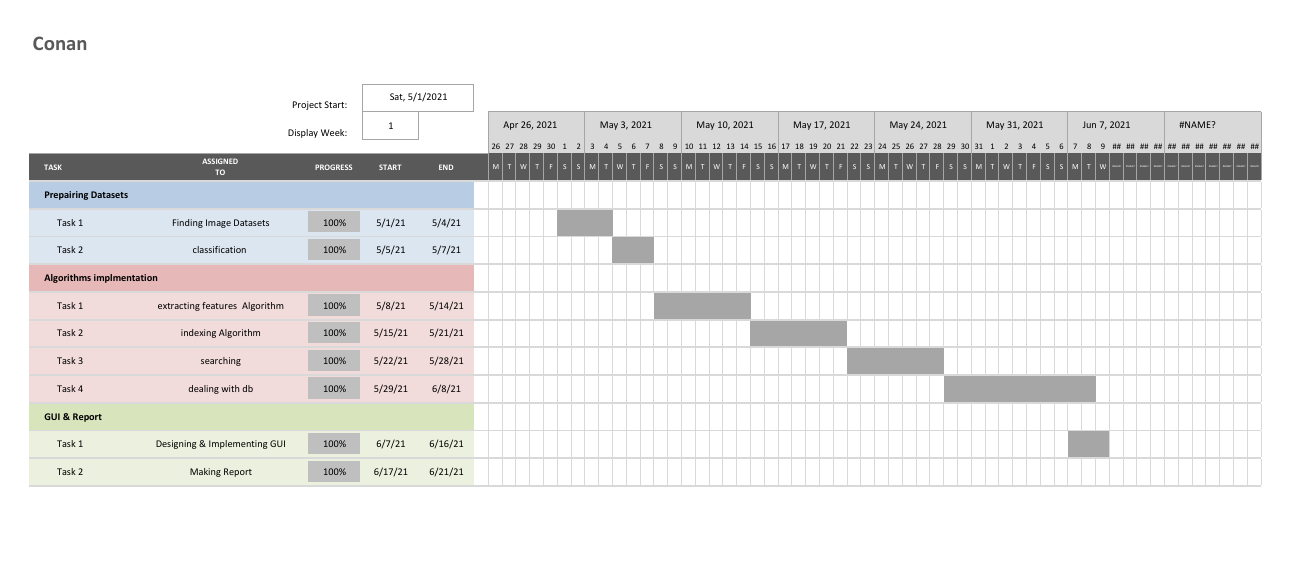
\includegraphics[width=140mm,height=80mm]{fig/5.png}
		\caption{time plan }
		\label{time plan}
	\end{figure}
	\pagebreak
	\section{System architecture}
		\begin{figure}[H]
		\centering
		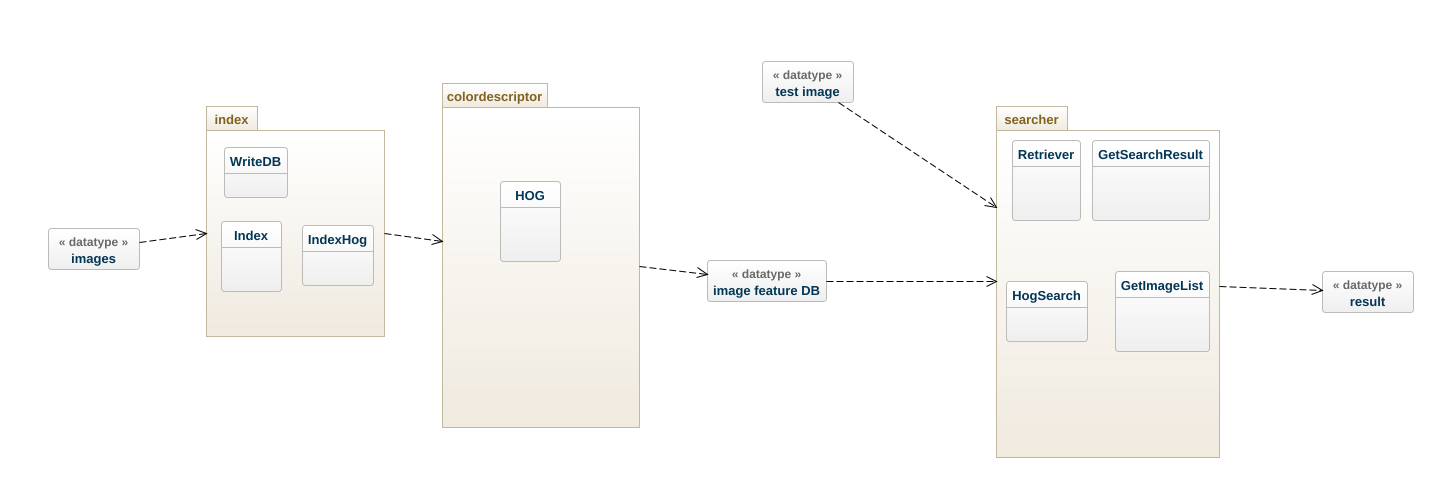
\includegraphics[width=140mm,height=80mm]{fig/22.png}
		\caption{System architecture class-diagram }
		\label{System architecture class-diagram}
	\end{figure}

\begin{figure}[H]
	\centering
	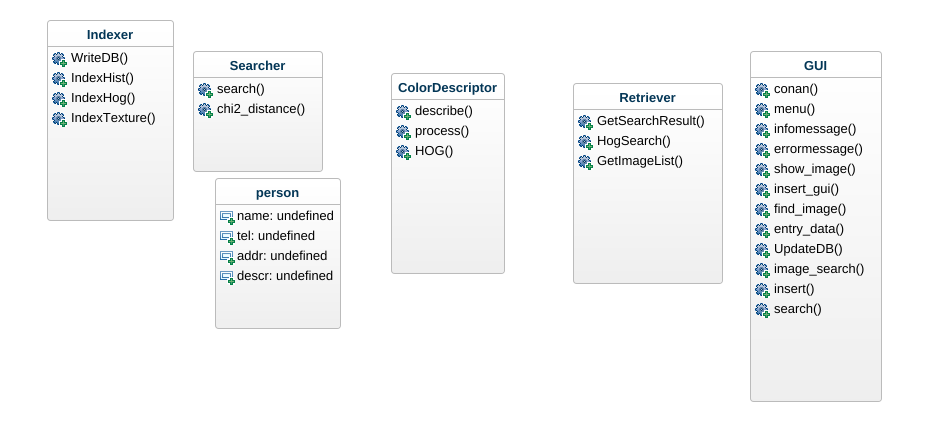
\includegraphics[width=140mm,height=80mm]{fig/23.png}
	\caption{class-diagram }
	\label{class-diagram}
\end{figure}

\pagebreak
	\section{database design}
	\begin{itemize}
		\item We implemented the schema in sqlite and store features in csv file which ID is the path of the image.
			\begin{figure}[H]
			\centering
			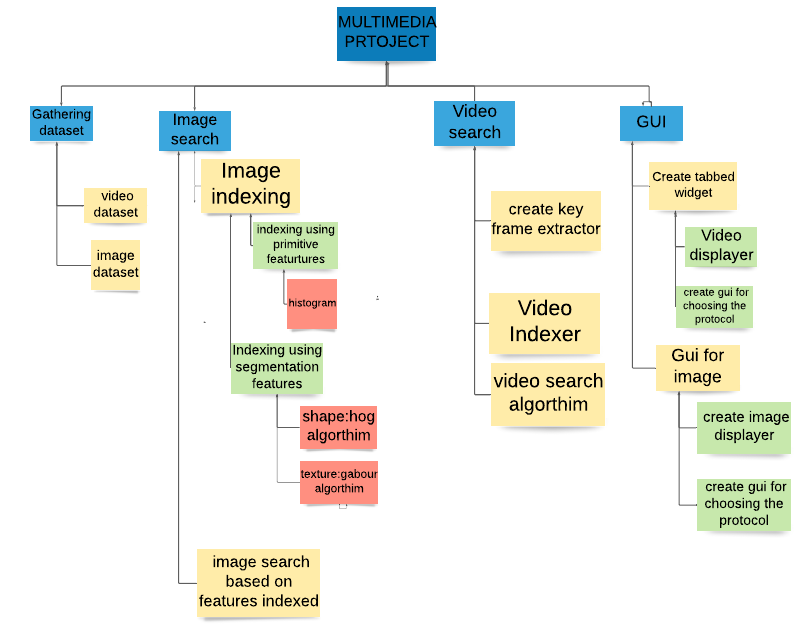
\includegraphics[width=120mm,height=60mm]{fig/25.png}
			\caption{DB EER Diagram }
			\label{DB EER Diagram }
		\end{figure}
	\begin{figure}[H]
		\centering
		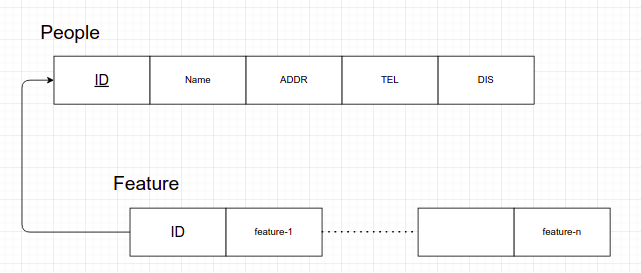
\includegraphics[width=120mm,height=60mm]{fig/24.png}
		\caption{Database Schema   }
		\label{Database Schema }
	\end{figure}
	\end{itemize}



\begin{figure}[H]
	\centering
	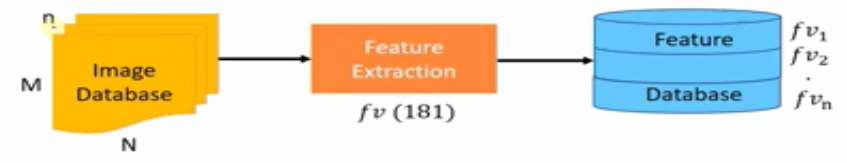
\includegraphics[width=120mm,height=60mm]{fig/21.png}
	\caption{image feature exract diagram }
	\label{image feature exract diagram}
\end{figure}
\begin{figure}[H]
	\centering
	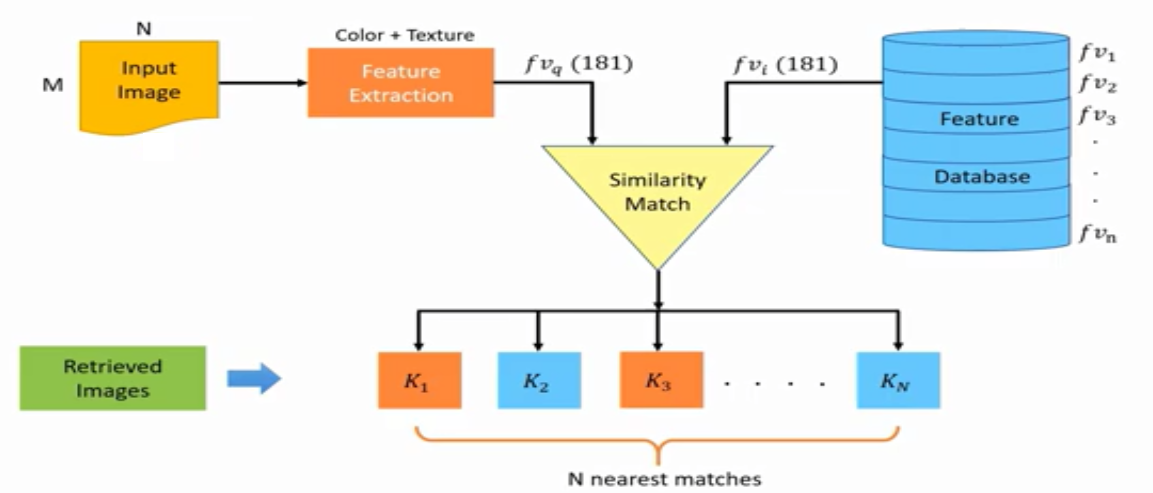
\includegraphics[width=120mm,height=60mm]{fig/20.png}
	\caption{image query diagram }
	\label{image query diagram}
\end{figure}
	\pagebreak
	\section{System design}
	\begin{enumerate}
		\item  \textbf{{\large system database}}\\
		in this project we have a database for images which has a CSV file each one store features for all techniques.
		
		
		\item \textbf{{\large user UI}} \\
		this is a GUI the user interact with to make queries.
		\item \textbf{{\large the processing part}}\\
		this part is responsible to process images according to the selected technique.
		\item \textbf{{\large  operating scenario}}\\
		 first we build our database for  images for all technique and then select from GUI  image search if image user select the technique and the image want to search with. all data from GUI is passed to the processing part to give results and print it in the GUI  
		
	\end{enumerate}
	
	
	 
	
	
	
	\pagebreak
	\section{Testing scenarios and results}
	\begin{figure}[H]
		\centering
		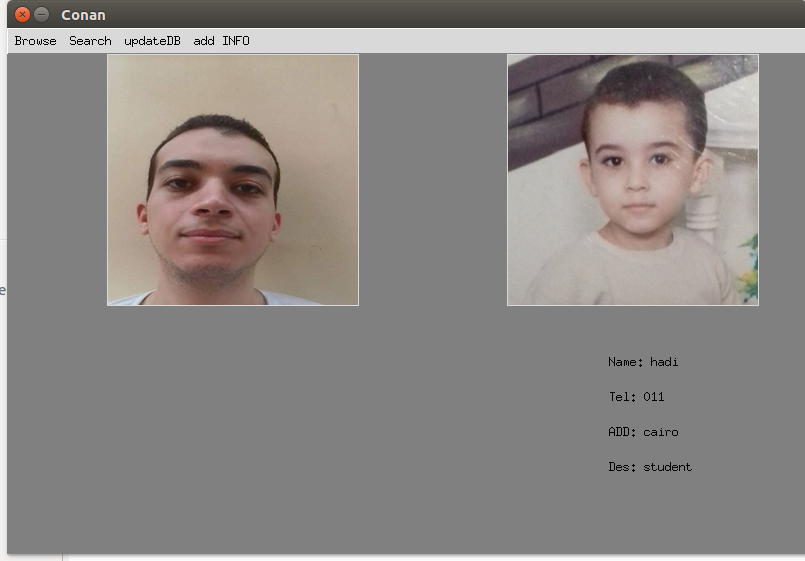
\includegraphics[width=120mm,height=60mm]{fig/17.png}
		%\caption{image feature exract diagram }
		%\label{image feature exract diagram}
	\end{figure}
	
	
	\begin{figure}[H]
	\centering
	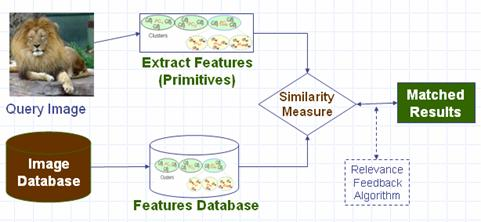
\includegraphics[width=120mm,height=60mm]{fig/18.png}
	%\caption{image feature exract diagram }
	%\label{image feature exract diagram}
\end{figure}
	\begin{figure}[H]
	\centering
	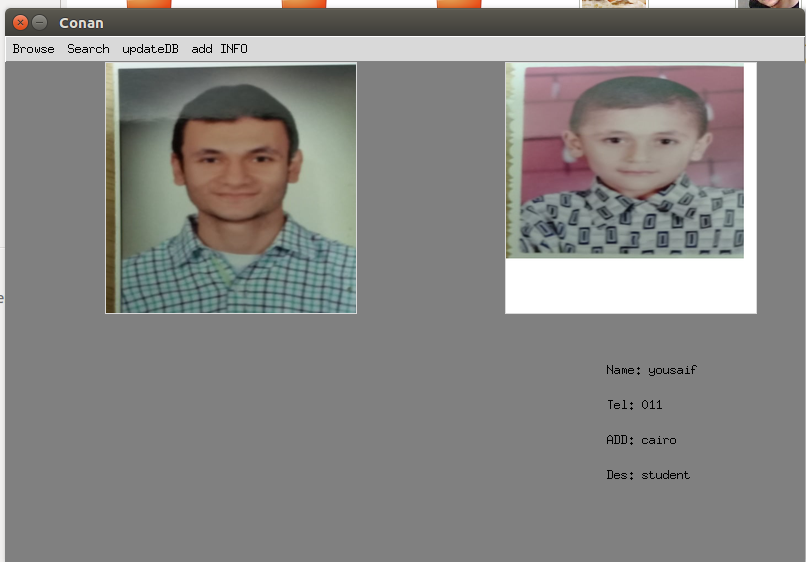
\includegraphics[width=120mm,height=60mm]{fig/14.png}
	%\caption{image feature exract diagram }
	%\label{image feature exract diagram}
\end{figure}
			\begin{figure}[H]
			\centering
			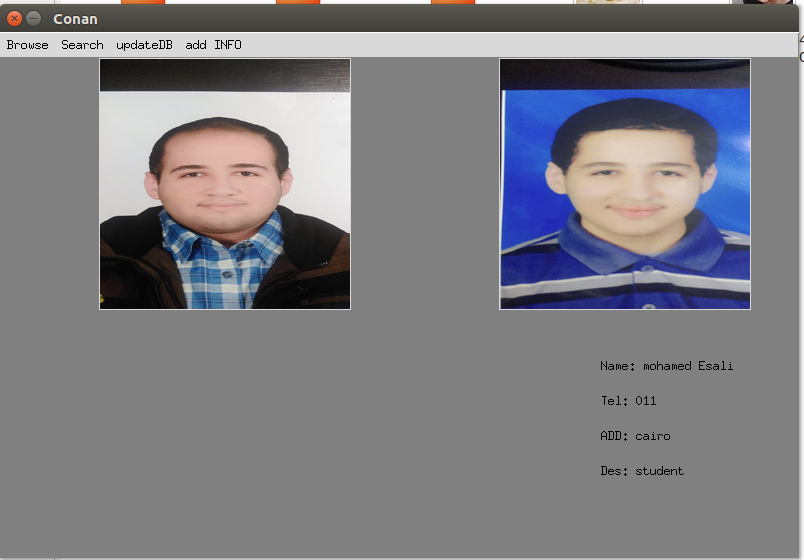
\includegraphics[width=120mm,height=60mm]{fig/15.png}
			%\caption{image feature exract diagram }
			%\label{image feature exract diagram}
		\end{figure}
	\begin{figure}[H]
	\centering
	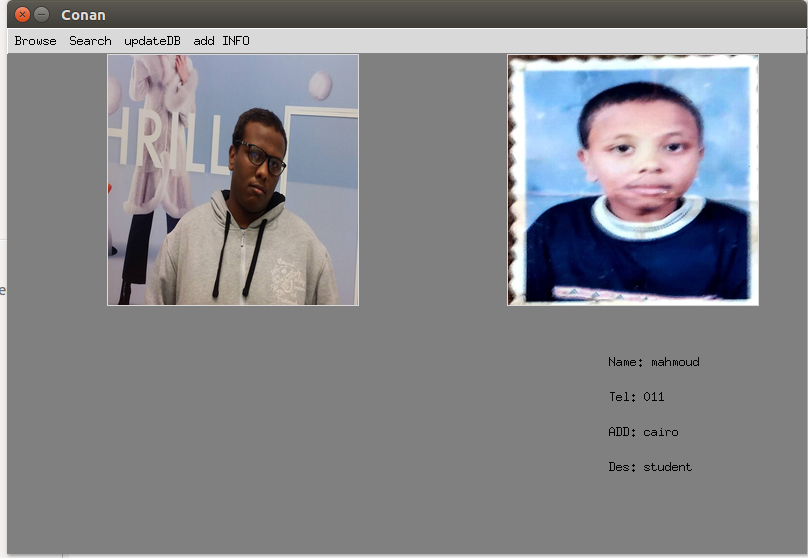
\includegraphics[width=120mm,height=60mm]{fig/16.png}
	%\caption{image feature exract diagram }
	%\label{image feature exract diagram}
\end{figure}
	\begin{figure}[H]
	\centering
	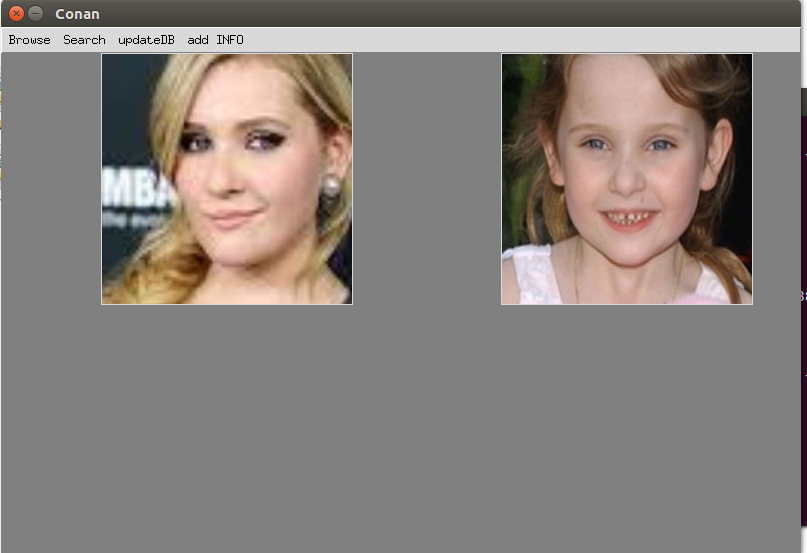
\includegraphics[width=120mm,height=60mm]{fig/10.png}
	%\caption{image feature exract diagram }
	%\label{image feature exract diagram}
\end{figure}
	\begin{figure}[H]
	\centering
	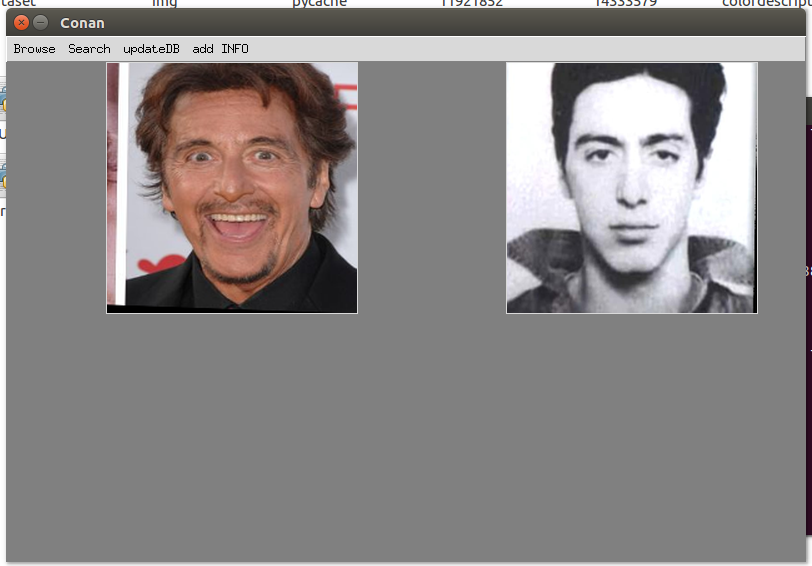
\includegraphics[width=120mm,height=60mm]{fig/11.png}
	%\caption{image feature exract diagram }
	%\label{image feature exract diagram}
\end{figure}
	\begin{figure}[H]
	\centering
	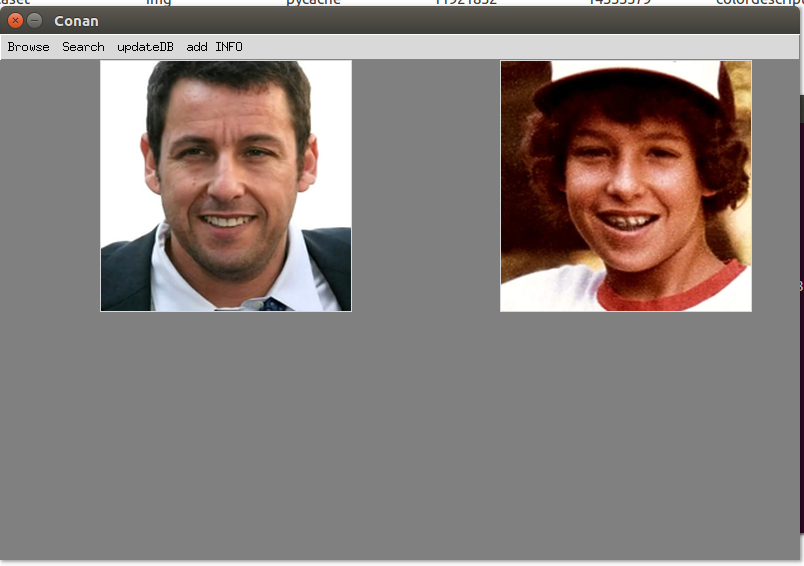
\includegraphics[width=120mm,height=60mm]{fig/12.png}
	%\caption{image feature exract diagram }
	%\label{image feature exract diagram}
\end{figure}
	\begin{figure}[H]
	\centering
	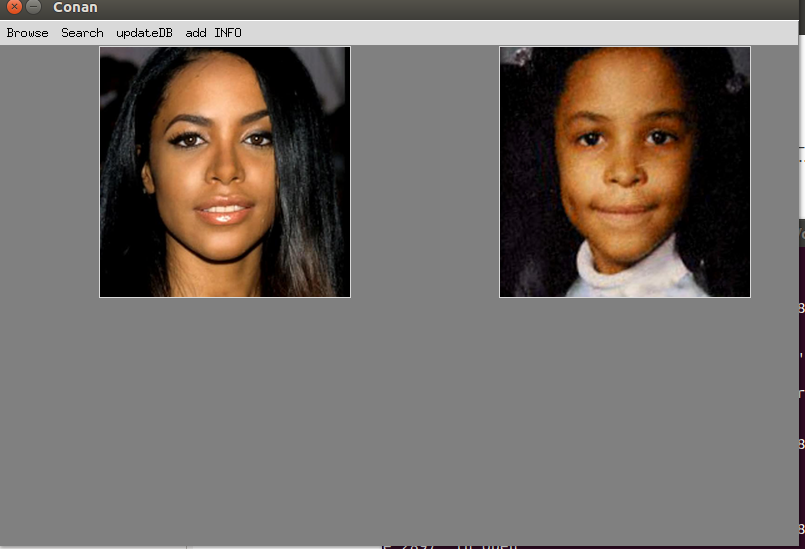
\includegraphics[width=120mm,height=60mm]{fig/13.png}
	%\caption{image feature exract diagram }
	%\label{image feature exract diagram}
\end{figure}
	\pagebreak
	\section{End user guide}
	\begin{enumerate}
		\item This is the primitive user interface.
			\begin{figure}[H]
			\centering
			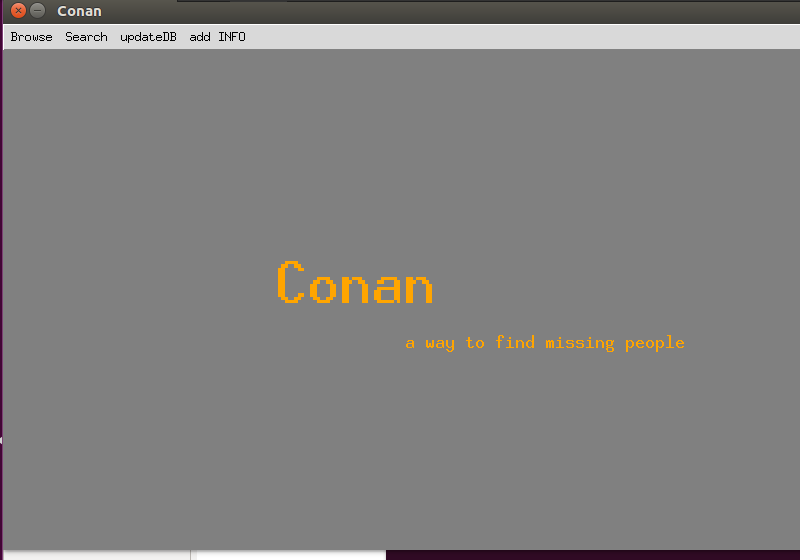
\includegraphics[width=120mm,height=60mm]{fig/00.png}
			%\caption{image feature exract diagram }
			%\label{image feature exract diagram}
		\end{figure}
		
	\pagebreak
	\item before to go in query we need to build database first so go from  updateDB
			
		\begin{figure}[H]
		\centering
		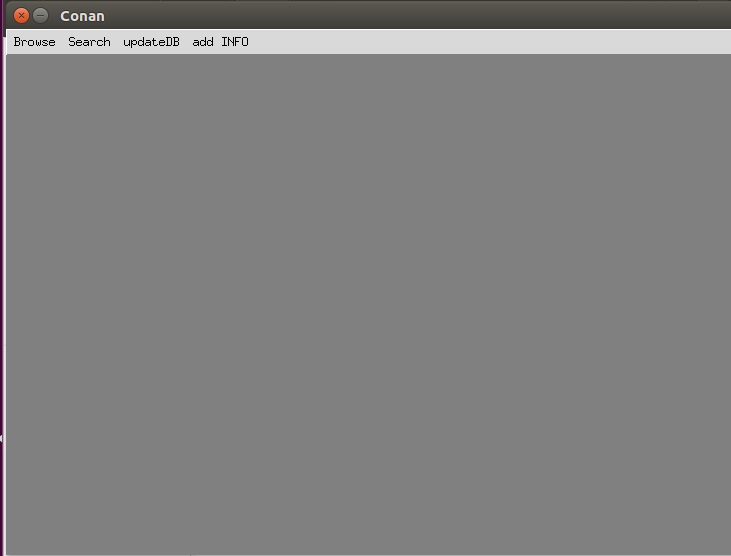
\includegraphics[width=120mm,height=60mm]{fig/01.png}
		%\caption{image feature exract diagram }
		%\label{image feature exract diagram}
	\end{figure}
		\item 	It may take a time and give you alert message for waiting.
	\begin{figure}[H]
	\centering
	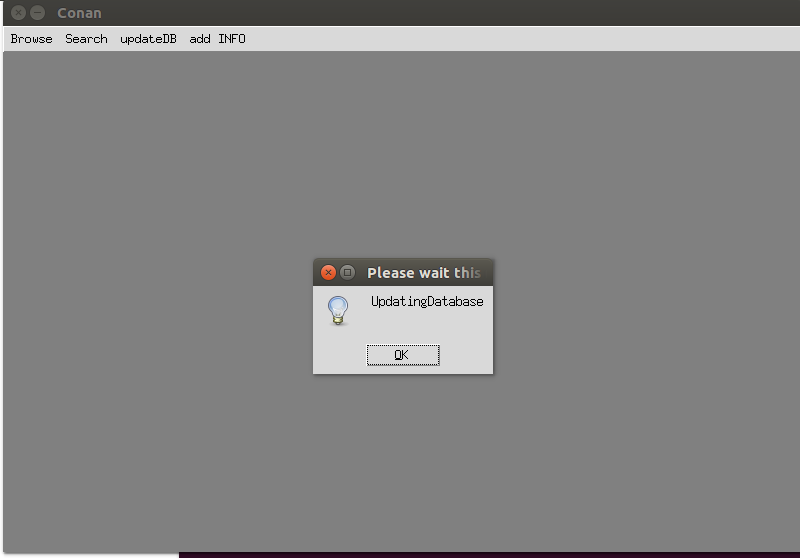
\includegraphics[width=120mm,height=60mm]{fig/2.png}
	%\caption{image feature exract diagram }
	%\label{image feature exract diagram}
\end{figure}
	
	
	\pagebreak
			\item 	When the database is finished updating, a message Database Status will appear.
		\begin{figure}[H]
		\centering
		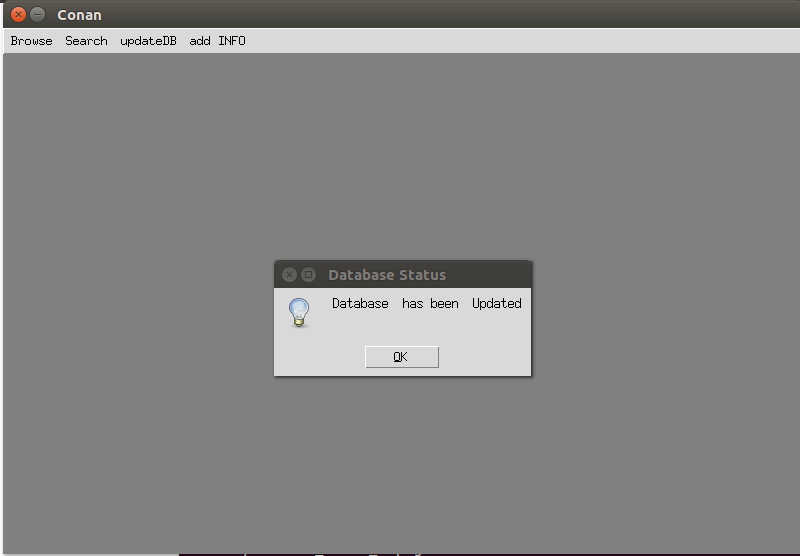
\includegraphics[width=120mm,height=60mm]{fig/3.png}
		%\caption{image feature exract diagram }
		%\label{image feature exract diagram}
	\end{figure}
	
	
	
	
	
	
	
	
		\item now we can search for any image we want From Browse choose Image ex Image. 
		
			\begin{figure}[H]
			\centering
			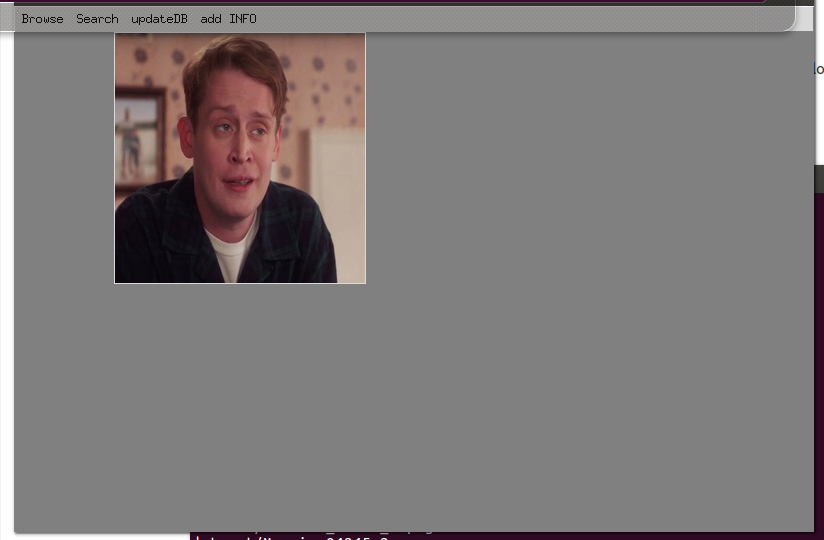
\includegraphics[width=120mm,height=60mm]{fig/4.png}
			%\caption{image feature exract diagram }
			%\label{image feature exract diagram}
		\end{figure}


\pagebreak
		\item 	to get the result Click on search button and the result will appear in the area for displaying results, and when you click at any result image it will be  standalone
		\begin{figure}[H]
		\centering
		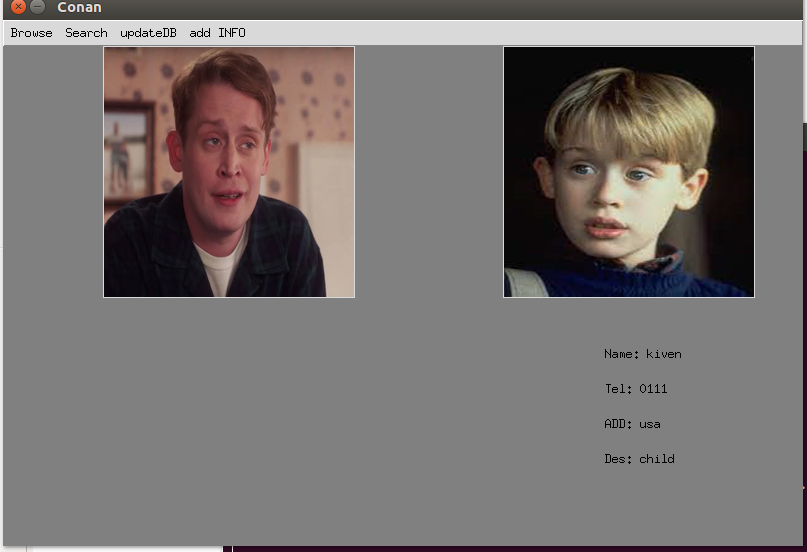
\includegraphics[width=120mm,height=60mm]{fig/05.png}
		%\caption{image feature exract diagram }
		%\label{image feature exract diagram}
	\end{figure}


	
	\item to enter information to image click to add INFO.
		
		 	\begin{figure}[H]
		 	\centering
		 	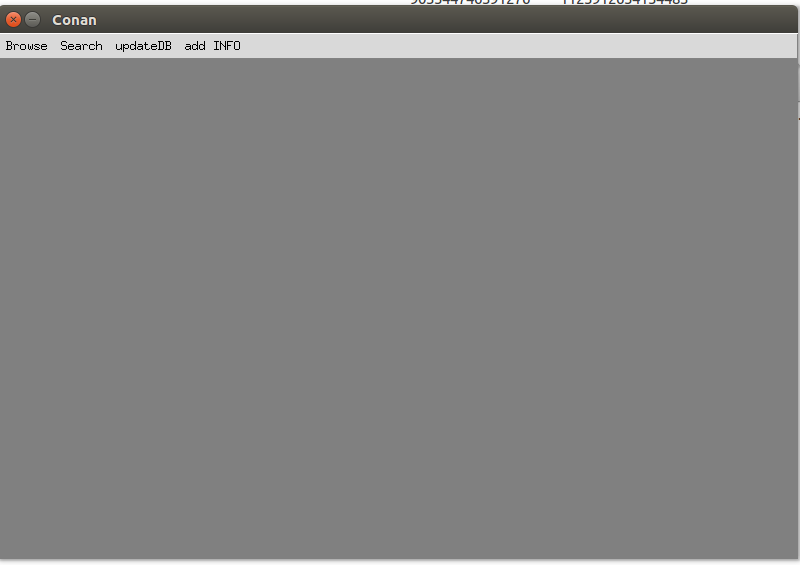
\includegraphics[width=120mm,height=60mm]{fig/06.png}
		 	%\caption{image feature exract diagram }
		 	%\label{image feature exract diagram}
		 \end{figure}
	
	
	\pagebreak
		\item 	another page will appear to enter information in diffrant fields.
			\begin{figure}[H]
			\centering
			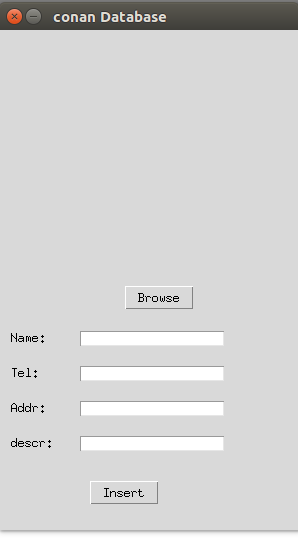
\includegraphics[width=60mm,height=60mm]{fig/7.png}
			%\caption{image feature exract diagram }
			%\label{image feature exract diagram}
		\end{figure}
	
		\begin{figure}[H]
		\centering
		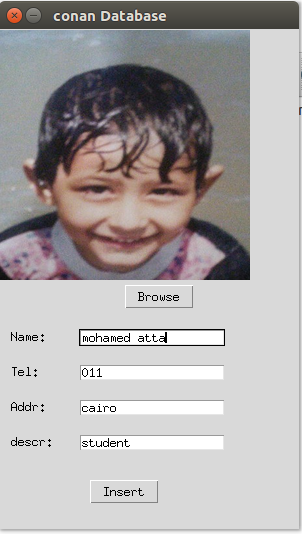
\includegraphics[width=60mm,height=60mm]{fig/09.png}
		%\caption{image feature exract diagram }
		%\label{image feature exract diagram}
	\end{figure}
		\begin{figure}[H]
		\centering
		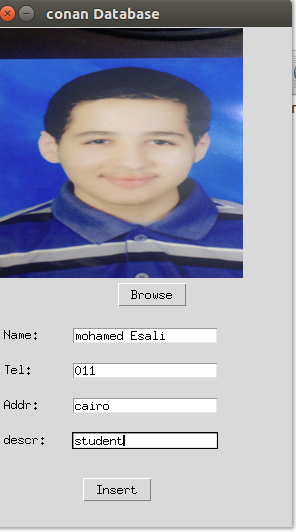
\includegraphics[width=60mm,height=60mm]{fig/08.png}
		%\caption{image feature exract diagram }
		%\label{image feature exract diagram}
	\end{figure}
		\begin{figure}[H]
		\centering
		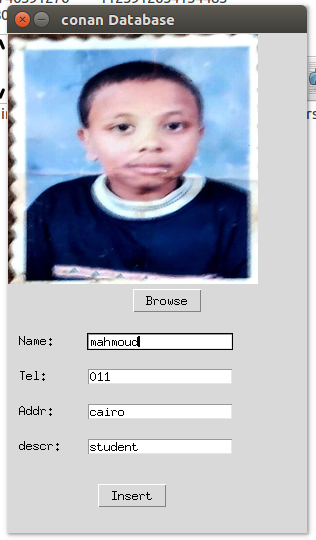
\includegraphics[width=50mm,height=60mm]{fig/07.png}
		%\caption{image feature exract diagram }
		%\label{image feature exract diagram}
	\end{figure}
	\begin{figure}[H]
	\centering
	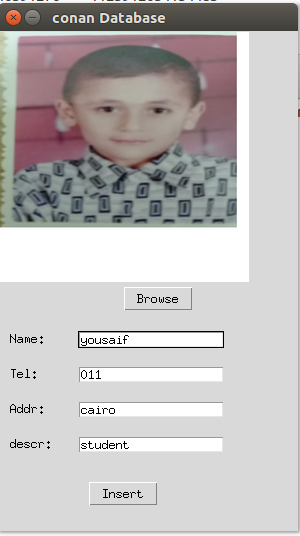
\includegraphics[width=60mm,height=50mm]{fig/6.png}
	%\caption{image feature exract diagram }
	%\label{image feature exract diagram}
\end{figure}
	\begin{figure}[H]
	\centering
	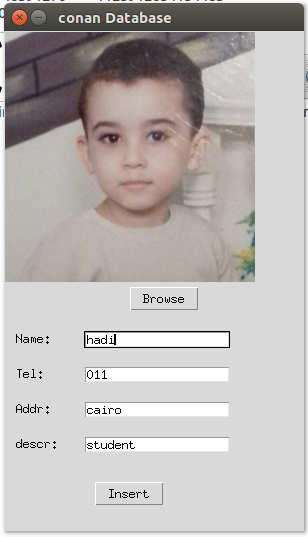
\includegraphics[width=60mm,height=50mm]{fig/04.png}
	%\caption{image feature exract diagram }
	%\label{image feature exract diagram}
\end{figure}
	\item 	When finshed  entering info , a message Status will appear.
		\begin{figure}[H]
		\centering
		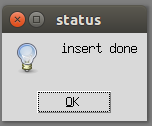
\includegraphics[width=60mm,height=20mm]{fig/8.png}
		%\caption{image feature exract diagram }
		%\label{image feature exract diagram}
	\end{figure}

						
	\end{enumerate}
\pagebreak

	\pagebreak
	\section{Conclusion}
	Finally, Conan application has been able to recongize missing people even if they have different ages.
	


	

	\pagebreak	
%	\addcontentsline{toc}{section}{References}
%	\bibliography{ref.bib} 
%	\bibliographystyle{ieeetr}
	
	
	\printglossary
\end{document}
